\section{Задание тканей при помощи ограничений} \label{ch2:connect} %название по-русски
	Ещё одна важная тема, которую необходимо осветить - способы задания различных мягких тел при помощи ограничений. Данная работа посвещена симуляции тканей, поэтому будут рассмотрены только способы их задания. В современных системах симуляции тканей используется два основных подхода: с помощью задания прямоугольной сетки и с использованием триангулированной геометрии.
	
	Для первого способа используются следующие ограничения:
	\begin{enumerate}[1.]
		\item Ограничение растяжения/структурное ограничение (Structural/streching). Определяется как ограничение \say{пружина}, соединяющее соседние частицы как показано на \firef{fig:structural}. Задает структуру всей ткани.
		\item Ограничение сдвига (Shear). Определяется как ограничение \say{пружина} соединяющее диагональные частицы как показано на \firef{fig:shear}. Вводится для корректной симуляции диагональных растяжений (\firef{fig:shear_blender}).
		\item Ограничение изгиба (Bending). Может определяться как ограничение угла \cite{wang2014angle} или как ограничение \say{пружина}, соединяющее частицы \say{через одну}, как показано на \firef{fig:bending}.
	\end{enumerate}
	
	\begin{figure}[ht!] 
		\center
		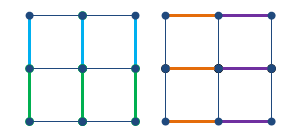
\includegraphics [scale=0.5] {my_folder/images//structural}
		\caption{Визуальная демонстрация структурных ограничений}
		\label{fig:structural}  
	\end{figure}
	
	\begin{figure}[ht!] 
		\center
		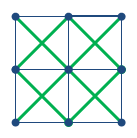
\includegraphics [scale=0.5] {my_folder/images//shear}
		\caption{Визуальная демонстрация ограничений сдвига}
		\label{fig:shear}  
	\end{figure}
	
	\begin{figure}[ht!] 
		\center
		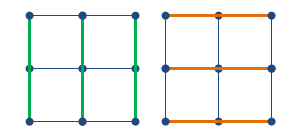
\includegraphics [scale=0.5] {my_folder/images//bending}
		\caption{Визуальная демонстрация ограничений изгиба}
		\label{fig:bending}  
	\end{figure}
	
	\begin{figure}[ht!] 
		\center
		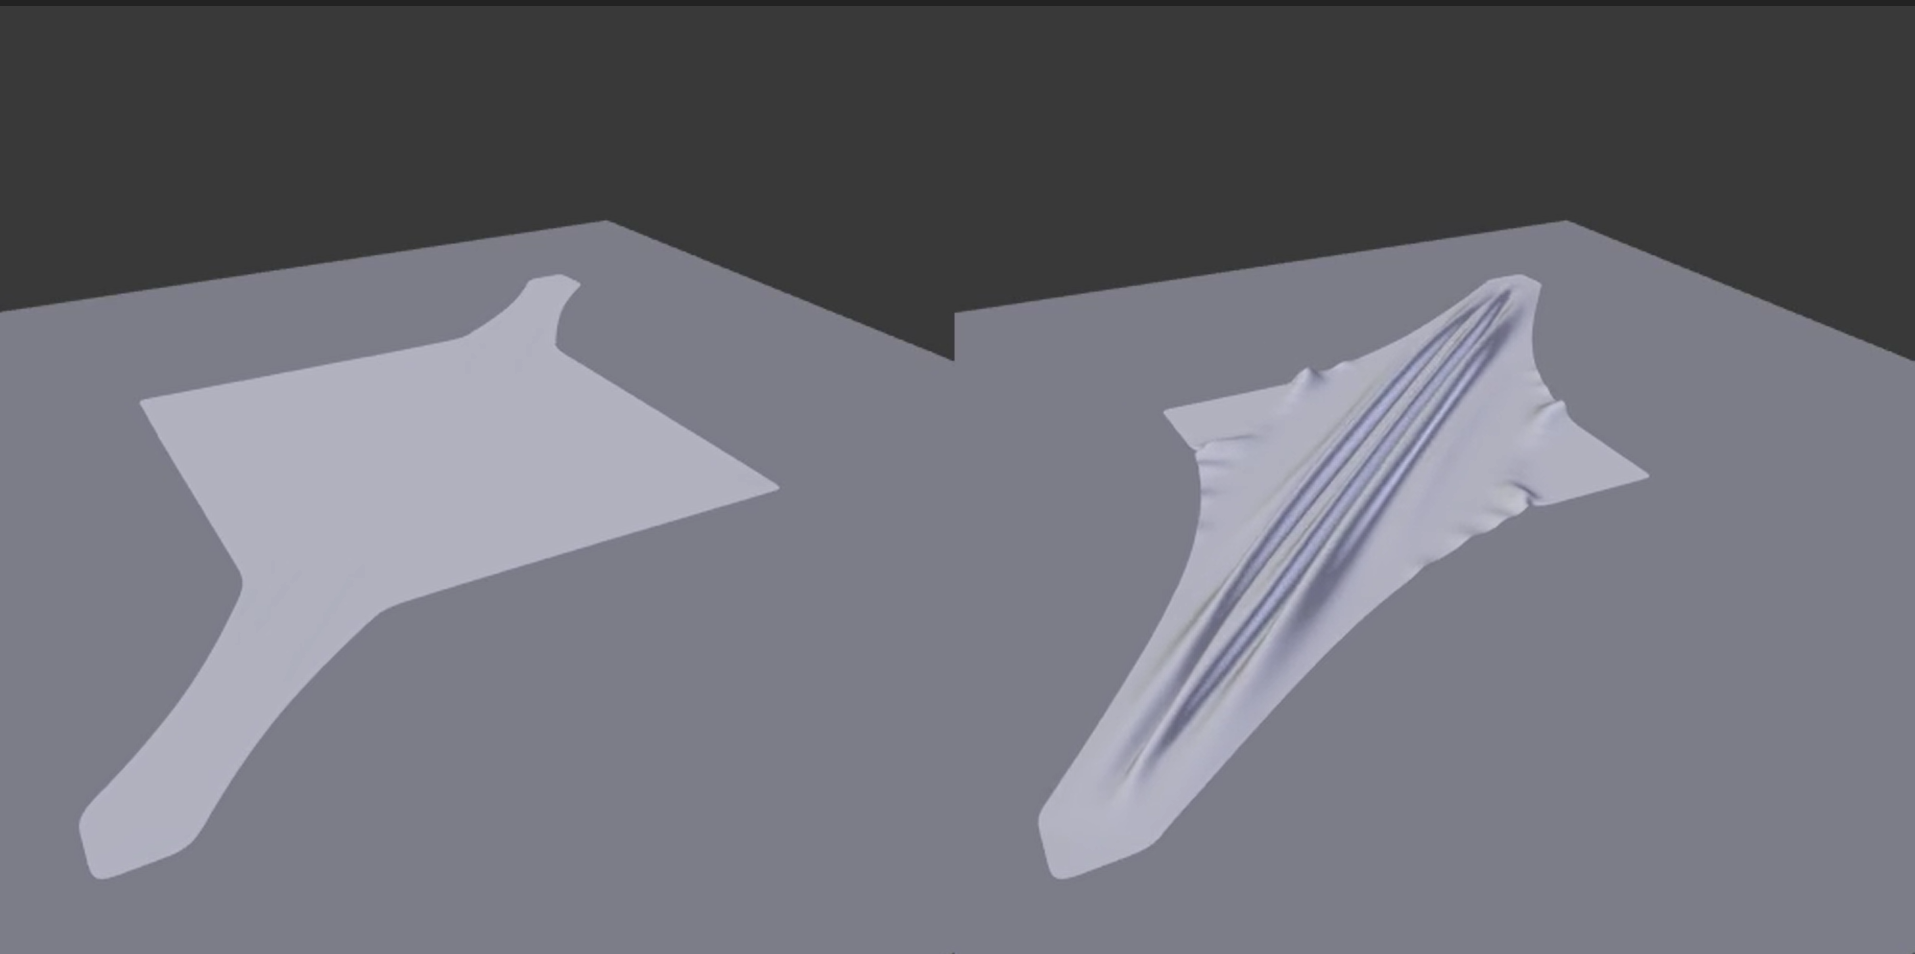
\includegraphics [scale=0.2] {my_folder/images//shear_blender}
		\caption{Сравнение тканей с отсутствием ограничения сдвига (слева) и наличием ограничения сдвига (справа)}
		\label{fig:shear_blender}  
	\end{figure}

	При использовании второго подхода, триангулированная геометрия проходит через предобработку, в которой вышеописанные ограничения (для прямоугольной сетки) накладываются на вершины триангулированной геометрии. Для этого триангулированная геометрия разбивается на прямоугольные сетки, а затем эти прямоугольные сетки \say{сшиваются} между собой при помощи структурных ограничений.
	
%% Вспомогательные команды - Additional commands
%
%\newpage % принудительное начало с новой страницы, использовать только в конце раздела
%\clearpage % осуществляется пакетом <<placeins>> в пределах секций
%\newpage\leavevmode\thispagestyle{empty}\newpage % 100 % начало новой страницы